\documentclass{article}[18pt]
\usepackage[utf8]{inputenc}
\usepackage[margin=0.7in]{geometry}
\usepackage{parselines} 
\usepackage{amsmath}
\usepackage{titlesec}
\usepackage{pgfplots}
\usepackage{graphicx}
\usepackage[english]{babel}
\usepackage{fancyhdr}
\usepackage{gensymb}
\usepackage{enumerate}
\usetikzlibrary{calc,shapes.geometric, arrows}
\tikzstyle{startstop} = [rectangle, rounded corners, minimum width=3cm, minimum height=1cm,text centered, draw=black, fill=red!30]
\tikzstyle{io} = [trapezium, trapezium left angle=70, trapezium right angle=110, minimum width=3cm, minimum height=1cm, text centered, draw=black, fill=blue!30]
\tikzstyle{process} = [rectangle, minimum width=3cm, minimum height=1cm, text centered, draw=black, fill=orange!30]
\tikzstyle{decision} = [diamond, minimum width=3cm, minimum height=1cm, text centered, draw=black, fill=green!30,text width=2cm]
\tikzstyle{arrow} = [thick,->,>=stealth]

\pgfplotsset{width=10cm,compat=1.9}

\titlespacing\section{0pt}{14pt plus 4pt minus 2pt}{0pt plus 2pt minus 2pt}
\newlength\tindent
\setlength{\tindent}{\parindent}
\setlength{\parindent}{0pt}
\renewcommand{\indent}{\hspace*{\tindent}}	
\newcommand{\cred}[1]{\color{red}#1}
\newcommand{\cblue}[1]{\color{blue}#1}
\newcommand{\cgreen}[1]{\color{green}#1}
\hyphenpenalty=10000
\pagestyle{fancy}
\fancyhf{}
\rhead{Sam Robbins 13SE}
\lhead{A Level Maths - D2}
\rfoot{Page \thepage}
\begin{document}
\begin{center}
\underline{\huge Transportation Problems}
\end{center}
\begin{obeylines}
\section{Terminology used in describing and modelling the transportation problem}
In order to solve transportation problems you need to consider:
\begin{itemize}
\item The capacity of each of the supply points - The quantity of goods that can be produced at each factory or held at each warehouse. Called \textbf{supply} or \textbf{stock}
\item The amount required at each of the demand points - The quantity of goods that are needed at each shop or by each customer. Called \textbf{demand} or \textbf{destination}
\item The unit cost of transporting goods from the supply points to the demand points
\end{itemize}
\subsection{Solving the transportation problem}
\begin{enumerate}
\item Find an initial solution that uses all the stock and meets all the demands
\item Calculate the total cost of this solution and see if it can be reduced by using routes not currently in the solution (if not then optimal)
\item If the cost can be reduced by a different route, put as many units across it as possible
\item Check to see if optimal, if not, go to 3
\item When no further savings are possible, an optimal solution has been found
\end{enumerate}
\section{Finding an initial solution to the transportation problem}
A method called the \textbf{north-west corner method} is used.
First, create a table with rows for source and columns for destination. Add demand at the bottom of each column and stock at the end of each row.
\begin{enumerate}
\item At the top left-hand corner of the table, allocate the maximum stock to meet demand
\item If stock is emptied, move down 1 and allocate
\item If demand is met, move 1 right and allocate
\item When all the stock is assigned and all the demands met, stop
\end{enumerate}
\end{obeylines}
\subsection{Example}
\textbf{What would be given in the question:}
\begin{center}
\begin{tabular}{ |c|c|c|c|c|c| }
\hline
&Depot W&Depot X&Depot Y&Depot Z&Stock\\
\hline
Supplier A&180&110&130&290&14\\
\hline
Supplier B&190&250&150&280&16\\
\hline
Supplier C&240&270&190&120&20\\
\hline
Demand&11&15&14&10&50\\ 
\hline
\end{tabular}
\end{center}
\textbf{Set up the table with stock and demand}
\begin{center}
\begin{tabular}{ |c|c|c|c|c|c| }
\hline
&W&X&Y&Z&Stock\\
\hline
A&&&&&14\\
\hline
B&&&&&16\\
\hline
C&&&&&20\\
\hline
Demand&11&15&14&10&50\\ 
\hline
\end{tabular}
\end{center}
\newpage
\textbf{Start by filling the top left corner}\\
11 is put here as it is the demand for \textbf{W} but does not exceed the stock of \textbf{A}
\begin{center}
\begin{tabular}{ |c|c|c|c|c|c| }
\hline
&W&X&Y&Z&Stock\\
\hline
A&11&&&&14\\
\hline
B&&&&&16\\
\hline
C&&&&&20\\
\hline
Demand&11&15&14&10&50\\ 
\hline
\end{tabular}
\end{center}
\textbf{Move 1 right as the demand has been satisfied}\\
3 is put here as it is the remainder of the stock of \textbf{A} and does not exceed the demand of \textbf{X}
\begin{center}
\begin{tabular}{ |c|c|c|c|c|c| }
\hline
&W&X&Y&Z&Stock\\
\hline
A&11&3&&&14\\
\hline
B&&&&&16\\
\hline
C&&&&&20\\
\hline
Demand&11&15&14&10&50\\ 
\hline
\end{tabular}
\end{center}
\textbf{Move 1 down as the stock of A has been exhausted}\\
12 is put here as it satisfies the demand for \textbf{X} but does not exceed the supply of \textbf{B}
\begin{center}
\begin{tabular}{ |c|c|c|c|c|c| }
\hline
&W&X&Y&Z&Stock\\
\hline
A&\textcolor{red}{11}&\textcolor{red}{3}&&&14\\
\hline
B&&\textcolor{red}{12}&&&16\\
\hline
C&&&&&20\\
\hline
Demand&11&15&14&10&50\\ 
\hline
\end{tabular}
\end{center}
\textbf{Move 1 right as the supply of B has not yet been exhausted}\\
4 is put here as it is the maximum \textbf{B} is able to supply and does not exceed the demand of \textbf{Y}
\begin{center}
\begin{tabular}{ |c|c|c|c|c|c| }
\hline
&W&X&Y&Z&Stock\\
\hline
A&\textcolor{red}{11}&\textcolor{red}{3}&&&14\\
\hline
B&&\textcolor{red}{12}&\textcolor{red}{4}&&16\\
\hline
C&&&&&20\\
\hline
Demand&11&15&14&10&50\\ 
\hline
\end{tabular}
\end{center}
\textbf{Move 1 down as the stock of B has been exhausted}\\
10 is put this as it meets the demand of \textbf{Y} without exceeding the stock of \textbf{C}
\begin{center}
\begin{tabular}{ |c|c|c|c|c|c| }
\hline
&W&X&Y&Z&Stock\\
\hline
A&\textcolor{red}{11}&\textcolor{red}{3}&&&14\\
\hline
B&&\textcolor{red}{12}&\textcolor{red}{4}&&16\\
\hline
C&&&\cred{10}&&20\\
\hline
Demand&11&15&14&10&50\\ 
\hline
\end{tabular}
\end{center}
\textbf{Move 1 right as the demand for Y has been met}\\
10 is put here as it meets the demand of \textbf{Z} and exhausts the stock of \textbf{C}
\begin{center}
\begin{tabular}{ |c|c|c|c|c|c| }
\hline
&W&X&Y&Z&Stock\\
\hline
A&\textcolor{red}{11}&\textcolor{red}{3}&&&14\\
\hline
B&&\textcolor{red}{12}&\textcolor{red}{4}&&16\\
\hline
C&&&\cred{10}&\cred{10}&20\\
\hline
Demand&11&15&14&10&50\\ 
\hline
\end{tabular}
\end{center}
\newpage
The total cost of transportation can then be found by multiplying the value in the square to be transported by the cost of that square.
\begin{center}
\begin{tabular}{ |c|c|c|c|c|c| }
\hline
&W&X&Y&Z&Stock\\
\hline
A&\textcolor{red}{11}$\times180$&\textcolor{red}{3}$\times110$&&&14\\
\hline
B&&\textcolor{red}{12}$\times250$&\textcolor{red}{4}$\times150$&&16\\
\hline
C&&&\textcolor{red}{10}$\times190$&\textcolor{red}{10}$\times120$&20\\
\hline
Demand&11&15&14&10&50\\ 
\hline
\end{tabular}
\end{center}
The sum of those multiplications is £9010, the cost of transportation.
\section{Unbalanced transportation problems}
When total supply$>$total demand, the problem is \textbf{unbalanced}\\
For an unbalanced transportation problem, add a dummy demand point with demand chosen to make demand and supply equal. All transportation costs of the dummy point is \textbf{zero}.
\subsection{Example}
\begin{center}
\begin{tabular}{ |c|c|c|c|c| }
\hline
&A&B&C&Supply\\
\hline
X&9&11&10&40\\
\hline
Y&10&8&12&60\\
\hline
Z&12&7&8&50\\
\hline
Demand&50&40&30&\\
\hline
\end{tabular}
\end{center}
Because 40+60+50>50+40+30 the problem is unbalanced.\\
\begin{center}
\begin{tabular}{ |c|c|c|c|c|c| }
\hline
&A&B&C&D&Supply\\
\hline
X&9&11&10&0&40\\
\hline
Y&10&8&12&0&60\\
\hline
Z&12&7&8&0&50\\
\hline
Demand&50&40&30&30&\\
\hline
\end{tabular}
\end{center}
The problem can then be solved as normal
\begin{center}
\begin{tabular}{ |c|c|c|c|c|c| }
\hline
&A&B&C&D&Supply\\
\hline
X&\cred{40}&&&&40\\
\hline
Y&\cred{10}&\cred{40}&\cred{10}&&60\\
\hline
Z&&&\cred{20}&\cred{30}&50\\
\hline
Demand&50&40&30&30&\\
\hline
\end{tabular}
\end{center}
\section{Degenerate solutions}
If the number of cells filled in a solution is less than suppliers+demanders-1 then the solution is \textbf{degenerate}.\\
\\
This happens when an entry, other than the last, satisfies both supply and demand at the same time, leading to the selector moving diagonally.\\
\\
The algorithm requires for n+m-1 cells to be used in every solution, so a zero needs to be placed in a currently unused cell.
\newpage
\subsection{Example}
\begin{center}
\begin{tabular}{ |c|c|c|c|c| }
\hline
&A&B&C&Supply\\
\hline
W&10&11&6&30\\
\hline
X&4&5&9&20\\
\hline
Y&3&8&7&35\\
\hline
Z&11&10&9&35\\
\hline
Demand&39&40&50&\\
\hline
\end{tabular}
\end{center}
This then gives the solution:
\begin{center}
\begin{tabular}{ |c|c|c|c|c| }
\hline
&A&B&C&Supply\\
\hline
W&\cred{30}&&&30\\
\hline
X&&\cred{20}&&20\\
\hline
Y&&\cred{20}&\cred{15}&35\\
\hline
Z&&&\cred{35}&35\\
\hline
Demand&39&40&50&\\
\hline
\end{tabular}
\end{center}
The problem with this is that it moves from AW to BX diagonally. This is solved by adding a zero in a place the selector could have moved after AW (BW or AX).
\begin{center}
\begin{tabular}{ |c|c|c|c|c| }
\hline
&A&B&C&Supply\\
\hline
W&\cred{30}&&&30\\
\hline
X&\textcolor{blue}{0}&\cred{20}&&20\\
\hline
Y&&\cred{20}&\cred{15}&35\\
\hline
Z&&&\cred{35}&35\\
\hline
Demand&39&40&50&\\
\hline
\end{tabular}
\end{center}
When doing this don't worry about where the zero goes, it can go in any empty space.
\section{Shadow costs}
Transportation costs are made up of two costs, one for source and one for destination, the cost of using that route is called the \textbf{shadow cost}.\\
\subsection{Description}
\begin{center}
\begin{tabular}{ |c|c|c|c|c|c| }
\hline
&W&X&Y&Z&Stock\\
\hline
A&\cred{180}&\cred{110}&&&14\\
\hline
B&&\cred{250}&\cred{150}&&16\\
\hline
C&&&\cred{190}&\cred{120}&20\\
\hline
Demand&11&15&14&10&50\\
\hline
\end{tabular}
\end{center}
Simultaneous equations can then be set up from this, for example:\\
S(A)+D(W)=180\\
S(A)+D(X)=110\\
S(B)+D(X)=250\\
As there are 5 equations and 6 unknowns relative costs need to be used.\\
\subsection{Method}
\begin{enumerate}
\item Set the source cost of the top left corner to zero
\item Move along the row and use \textbf{cost of destination =total cost-cost of supply}
\item When all the costs for that row have been found, move down one row and use the data already found to determine the supply cost
\item Repeat step 2 and step 3 until all costs have been found.
\end{enumerate}
\subsection{Example}
\textbf{Set up a table with space for shadow costs}\\
\begin{center}
\begin{tabular}{ |c|c|c|c|c|c|c| }
\hline
Shadow costs&&&&&&\\
\hline
&&Depot W&Depot X&Depot Y&Depot Z&Stock\\
\hline
&Supply A&\cred{180}&\cred{110}&&&14\\
\hline
&Supply B&&\cred{250}&\cred{150}&&16\\
\hline
&Supply C&&&\cred{190}&\cred{120}&20\\
\hline
&Demand&11&15&14&10&50\\
\hline
\end{tabular}
\end{center}
\textbf{Set the cost of source for the top left corner to zero and use to fill out the depot cost for the row}\\
\begin{center}
\begin{tabular}{ |c|c|c|c|c|c|c| }
\hline
Shadow costs&&180&110&&&\\
\hline
&&Depot W&Depot X&Depot Y&Depot Z&Stock\\
\hline
0&Supply A&\cred{180}&\cred{110}&&&14\\
\hline
&Supply B&&\cred{250}&\cred{150}&&16\\
\hline
&Supply C&&&\cred{190}&\cred{120}&20\\
\hline
&Demand&11&15&14&10&50\\
\hline
\end{tabular}
\end{center}
\textbf{Move 1 row down and use filled out values to determine all the values for that row}
\begin{center}
\begin{tabular}{ |c|c|c|c|c|c|c| }
\hline
Shadow costs&&180&110&10&&\\
\hline
&&Depot W&Depot X&Depot Y&Depot Z&Stock\\
\hline
0&Supply A&\cred{180}&\cred{110}&&&14\\
\hline
140&Supply B&&\cred{250}&\cred{150}&&16\\
\hline
&Supply C&&&\cred{190}&\cred{120}&20\\
\hline
&Demand&11&15&14&10&50\\
\hline
\end{tabular}
\end{center}
\textbf{Repeat step above}
\begin{center}
\begin{tabular}{ |c|c|c|c|c|c|c| }
\hline
Shadow costs&&180&110&10&-60&\\
\hline
&&Depot W&Depot X&Depot Y&Depot Z&Stock\\
\hline
0&Supply A&\cred{180}&\cred{110}&&&14\\
\hline
140&Supply B&&\cred{250}&\cred{150}&&16\\
\hline
180&Supply C&&&\cred{190}&\cred{120}&20\\
\hline
&Demand&11&15&14&10&50\\
\hline
\end{tabular}
\end{center}
\textbf{Write all the costs individually}\\
S(A)=0\\
S(B)=140\\
S(C)=180\\
D(W)=180\\
D(X)=110\\
D(Y)=10\\
D(Z)=-60\\
\section{Improvement indices}
Improvement indices look at each unused route and calculate the reduction in cost by using that route.\\
The formula for an improvement index for PX= $\mathbf{I_{PQ}=C(PQ)-S(P)-D(Q)}$\\
The route with the most negative improvement index will be introduced to the solution.\\
The route introduced to the solution is called the \textbf{entering cell} and the route it replaces is called the \textbf{exiting cell}.\\
If there are two equal entering or exiting cells choose either.\\
If there are no negative improvement indices the solution is \textbf{optimal}.
\subsection{Example}
\textbf{Start with the shadow costs}
\begin{center}
\begin{tabular}{ |c|c|c|c|c|c|c| }
\hline
Shadow costs&&180&110&10&-60&\\
\hline
&&Depot W&Depot X&Depot Y&Depot Z&Stock\\
\hline
0&Supply A&\cred{180}&\cred{110}&&&14\\
\hline
140&Supply B&&\cred{250}&\cred{150}&&16\\
\hline
180&Supply C&&&\cred{190}&\cred{120}&20\\
\hline
&Demand&11&15&14&10&50\\
\hline
\end{tabular}
\end{center}
\textbf{Use the formula to calculate improvement indices}\\
\begin{center}
\begin{tabular}{ |c|c|c|c|c|c|c| }
\hline
Shadow costs&&180&110&10&-60&\\
\hline
&&Depot W&Depot X&Depot Y&Depot Z&Stock\\
\hline
0&Supply A&\cred{0}&\cred{0}&\cblue{120}&\cblue{350}&14\\
\hline
140&Supply B&\cblue{-130}&\cred{0}&\cred{0}&\cblue{200}&16\\
\hline
180&Supply C&\cblue{-120}&\cblue{20}&\cred{0}&\cred{0}&20\\
\hline
&Demand&11&15&14&10&50\\
\hline
\end{tabular}
\end{center}
This shows that BW is the entering cell as it has the lowest improvement index.
\section{Stepping stone method}
The stepping stone method is a method to find a more optimal solution given improvement indices.\\
This looks for a cycle of adjustments, increasing the value in one cell and reducing in the next and so on.
\subsection{Method}
\begin{enumerate}
\item Create a cycle of adjustments with the rules:
\begin{enumerate}
\item Within any row or column there can only be one increasing and one decreasing cell
\item With the exception of the entering cell, adjustments can only be made to filled cells
\end{enumerate}
\item Once the cycle of adjustments has been found, transfer the maximum number of units through this cycle. This will be equal to the smallest number in the decreasing cells to avoid negative units.
\item Adjust the solution to incorporate this solution
\end{enumerate}
\subsection{Example}
\textbf{Start with the initial solution}
\begin{center}
\begin{tabular}{ |c|c|c|c|c|c| }
\hline
&W&X&Y&Z&Stock\\
\hline
A&\cblue{11}&\cblue{3}&&&14\\
\hline
B&&\cblue{12}&\cblue{4}&&16\\
\hline
C&&&\cblue{10}&\cblue{10}&20\\
\hline
Demand&11&15&14&10&50\\ 
\hline
\end{tabular}
\end{center}
\textbf{Insert a theta in the value with the most negative improvement index}
\begin{center}
\begin{tabular}{ |c|c|c|c|c|c| }
\hline
&W&X&Y&Z&Stock\\
\hline
A&\cblue{11}&\cblue{3}&&&14\\
\hline
B&\cgreen{$\theta}$&\cblue{12}&\cblue{4}&&16\\
\hline
C&&&\cblue{10}&\cblue{10}&20\\
\hline
Demand&11&15&14&10&50\\ 
\hline
\end{tabular}
\end{center}
\textbf{Subtract theta from AW to keep the demand at W correct. Then add theta to AX to keep the stock at AX correct, finally subtract theta from BX to keep the demand at X correct}
\begin{center}
\begin{tabular}{ |c|c|c|c|c|c| }
\hline
&W&X&Y&Z&Stock\\
\hline
A&\cred{$11-\theta$}&\cgreen{$3+\theta$}&&&14\\
\hline
B&\cgreen{$\theta}$&\cred{$12-\theta$}&\cblue{4}&&16\\
\hline
C&&&\cblue{10}&\cblue{10}&20\\
\hline
Demand&11&15&14&10&50\\ 
\hline
\end{tabular}
\end{center}
\textbf{Substitute 11 for theta as that is the smallest value in a decreasing cell}
\begin{center}
\begin{tabular}{ |c|c|c|c|c|c| }
\hline
&W&X&Y&Z&Stock\\
\hline
A&\cred{$11-11$}&\cgreen{$3+11$}&&&14\\
\hline
B&\cgreen{$11$}&\cred{$12-11$}&\cblue{4}&&16\\
\hline
C&&&\cblue{10}&\cblue{10}&20\\
\hline
Demand&11&15&14&10&50\\ 
\hline
\end{tabular}
\end{center}
\textbf{Write the improved solution and find the cost}

\begin{center}
\begin{tabular}{ |c|c|c|c|c|c| }
\hline
&W&X&Y&Z&Stock\\
\hline
A&&\cblue{$14$}&&&14\\
\hline
B&\cblue{$11$}&\cblue{$1$}&\cblue{4}&&16\\
\hline
C&&&\cblue{10}&\cblue{10}&20\\
\hline
Demand&11&15&14&10&50\\ 
\hline
\end{tabular}
\end{center}
The cost of this is £7580, a reduction from the initial solution.\\
\textbf{AW has become empty, meaning it is the exiting cell}\\
\textbf{To find an optimal solution, new shadow costs and improvement indices would need to be found}
\newpage
\section{Finding an initial solution to the transportation problem}
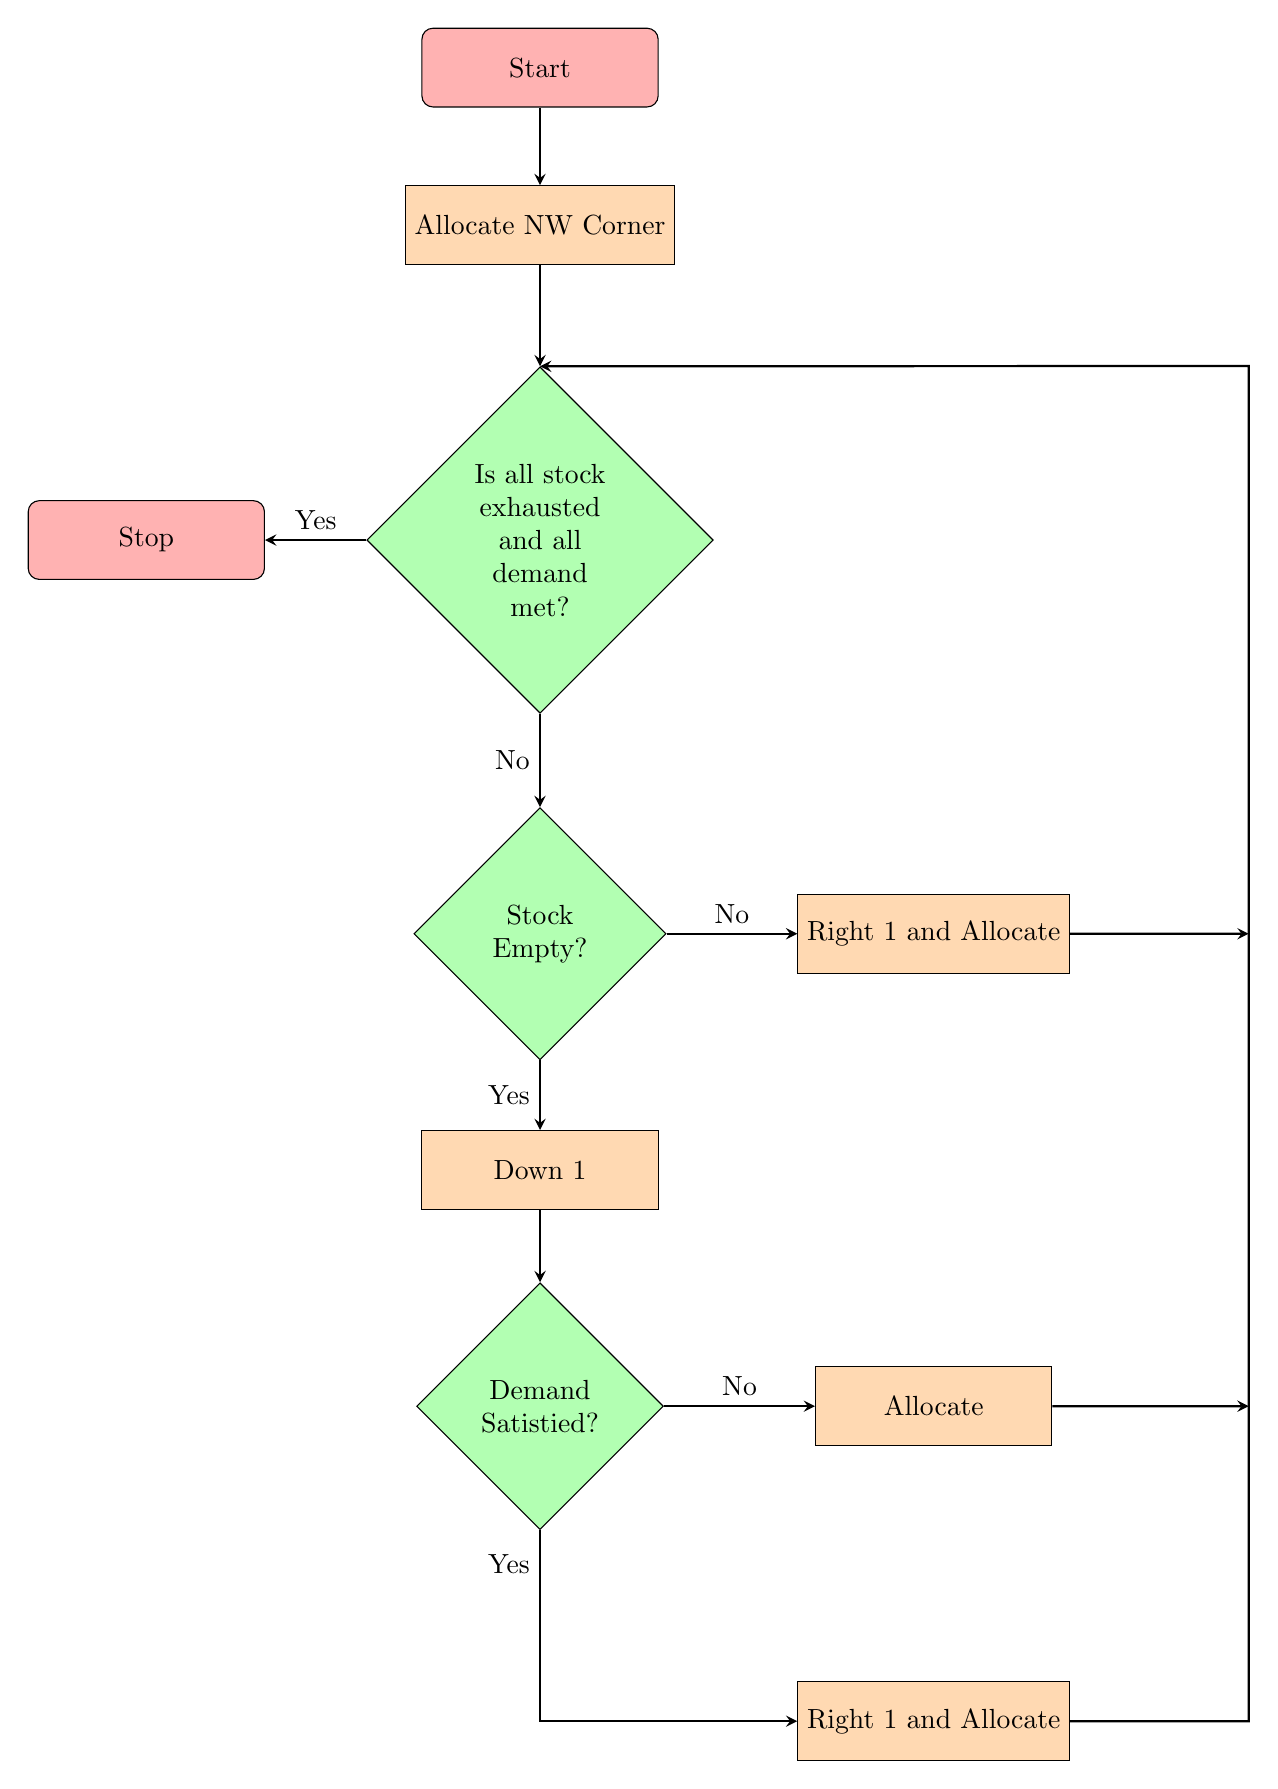
\begin{tikzpicture}[node distance=2cm]
\node (start) [startstop] {Start};
\node (pro1) [process, below of=start] {Allocate NW Corner};
\node (dec1) [decision, below of=pro1, yshift=-2cm] {Is all stock exhausted and all demand met?};
\node (dec2) [decision, below of=dec1, yshift=-3cm] {Stock Empty?};

\node (pro2) [process, below of=dec2,yshift=-1cm] {Down 1};
\node (pro3) [process, right of=dec2,xshift=3cm] {Right 1 and Allocate};

\node (dec3) [decision, below of=pro2, yshift=-1cm] {Demand Satistied?};
\node (pro4) [process, right of=dec3,xshift=3cm] {Allocate};
\node (pro5) [process, right of=dec3,xshift=3cm,yshift=-4cm] {Right 1 and Allocate};
\node (stop) [startstop,left of=dec1,xshift=-3cm] {Stop};

\draw [arrow] (start) -- (pro1);
\draw [arrow] (pro1) -- (dec1);
\draw [arrow] (pro2) -- (dec3);
\draw [arrow] (dec1) -- node[anchor=south] {Yes} (stop);
\draw [arrow] (dec1) -- node[anchor=east] {No} (dec2);
\draw [arrow] (dec2) -- node[anchor=east] {Yes} (pro2);
\draw [arrow] (dec2) -- node[anchor=south] {No} (pro3);

\draw [arrow] (dec3) |- node[anchor=east,yshift=2cm] {Yes} (pro5);
\draw [arrow] (dec3) -- node[anchor=south] {No} (pro4);
\draw [arrow] (pro5.east) --  (9,-21)-- (9,-3.79)-- (dec1.north);
\draw [arrow] (pro3.east) -- (9,-11);
\draw [arrow] (pro4.east) -- (9,-17);
\end{tikzpicture}
\newpage
\section{Finding an improvement to the initial solution}

\end{document}